%\documentclass[12pt, a4paper]{article}
\documentclass[runningheads]{llncs}
\usepackage{graphicx}
\usepackage{wrapfig}
\usepackage{subfigure}
\usepackage{multirow}
\usepackage{hyperref}
\usepackage{amsmath}
\usepackage{amssymb}
% \usepackage{ngerman}
\usepackage[ansinew]{inputenc}
\usepackage[left=2.5cm,top=2.5cm]{geometry}

\renewcommand\UrlFont{\color{blue}\rmfamily}

\begin{document}

\title{The effect of commen network problems on students academic performance in an elearning-Environment \thanks{Supported by Goethe University Frankfurt a. Main}}

\author{Lucas Laub\inst{1}\orcidID{6621331} \and
Second Author\inst{2}\orcidID{1111-2222-3333-4444}}

\institute{Goethe University Frankfurt, 60323 Frankfurt a. Main, Germany.}

\maketitle

\begin{abstract}
In the current light of the pandemic the worldwide use
of eLearning-Software experienced an unpresented boom.
We state the question how commen network problems influence
the academic performance in an eLearning-Environment.
To provide answers an online questionnaire with deliberate
technical difficulties was constructed. Evaluating the performance
of the test and controll group did not show any significant
differences.
\keywords{eLearning  \and Online-Learning \and academic performance.}
\end{abstract}


\section{Introduction}
\section{Materials and Methodes}
\subsection{Preperations}
The experiment was conducted by creating a software implementing Fig.~\ref{fig1}.
This software allowed the tracking of {\itshape technical problems} introduced by
the software itself as well as the points and answers scored by each participant.
Additianaly a room with an adequat number of computers with a fiber-connection
to the server are needed, to rule out uncontrolled network problems.
Half of the cumputers are manipulated and simulate the network problems with the
use of the software.

\begin{figure}
    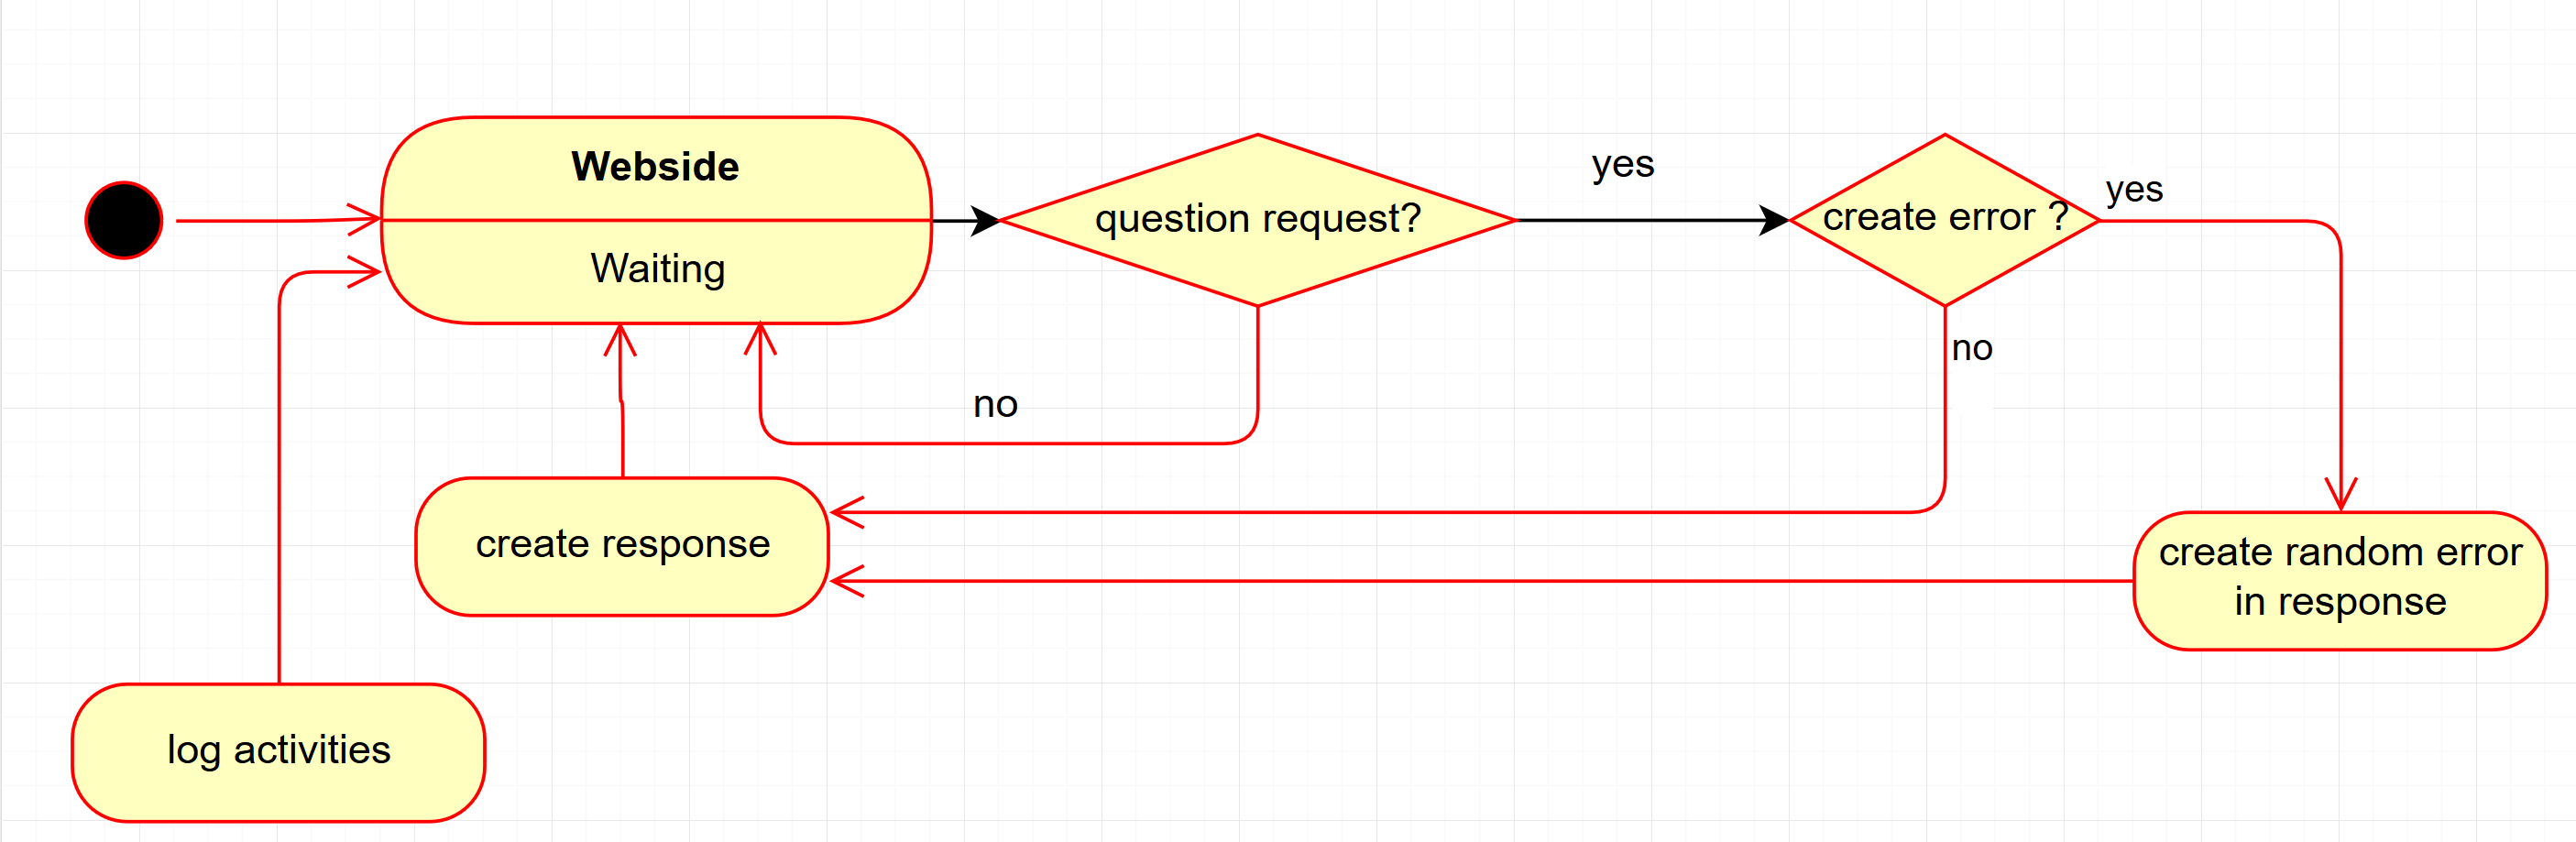
\includegraphics[width=\textwidth]{UML Prototyp.PNG}
    \caption{A logic flow chart , representing how an implementation could operate.
    The black circle is the user interacting with the software. The webside would
    consist of two parts. A frontend handling user interaction and the creation of {\itshape bugs}.
    The backend responsible for saving the collected data and ensuring the frontend
    remains operationale.} \label{fig1}
\end{figure}

\subsection{Participants}
The participants are students of the 5 grade and consist of two groups the controll group [CG] and
the test group [TG]. Each group is made up by 50 girls and 50 boys for a total of 200 participants.
It should be ensured that both groups prior to the experiment perform academicly similar, if not a
comparison post experiment will be difficult.

\section{Results}
\section{Discussion}
\section{Conclusion}
\section{Refernces}
\end{document}
